\documentclass[12pt, a4paper]{article}

\usepackage[left = 35mm, right = 25mm, top = 25mm, bottom = 25mm]{geometry}
\usepackage{titlesec}
\usepackage{hyperref}
\usepackage{graphicx}
\usepackage{setspace}
\usepackage{listings}
\usepackage{float}
\usepackage{textcomp}
\usepackage{array}
\usepackage{caption}
\usepackage[backend=biber, style=numeric]{biblatex}
\addbibresource{latex_test.bib}

\renewcommand{\appendixname}{Appendix}

\lstset{
  frame=lines,
  showstringspaces=false,
  columns=flexible,
  basicstyle={\small\ttfamily},
  numbers=none,
  breaklines=true,
  breakatwhitespace=true,
  tabsize=3,
}

\hyphenpenalty=10000
\exhyphenpenalty=10000

\titleclass{\subsubsubsection}{straight}[\subsection]

\newcounter{subsubsubsection}[subsubsection]
\renewcommand\thesubsubsubsection{\thesubsubsection.\arabic{subsubsubsection}}
\renewcommand\theparagraph{\thesubsubsubsection.\arabic{paragraph}} % optional; useful if paragraphs are to be numbered

\titleformat{\subsubsubsection}
  {\normalfont\normalsize\bfseries}{\thesubsubsubsection}{1em}{}
\titlespacing*{\subsubsubsection}
{0pt}{3.25ex plus 1ex minus .2ex}{1.5ex plus .2ex}

\makeatletter
\renewcommand\paragraph{\@startsection{paragraph}{5}{\parindent}%
  {0ex \@plus1ex \@minus.2ex}%
  {-1em}%
  {\normalfont\normalsize\bfseries}}
\renewcommand\subparagraph{\@startsection{subparagraph}{6}{\parindent}%
  {0ex \@plus1ex \@minus.2ex}%
  {-1em}%
  {\normalfont\normalsize\bfseries}}
\def\toclevel@subsubsubsection{4}
\def\toclevel@paragraph{5}
\def\toclevel@paragraph{6}
\def\l@subsubsubsection{\@dottedtocline{4}{7em}{4em}}
\def\l@paragraph{\@dottedtocline{5}{10em}{5em}}
\def\l@subparagraph{\@dottedtocline{6}{14em}{6em}}
\makeatother

\setcounter{secnumdepth}{4}
\setcounter{tocdepth}{4}
\spacing{1.5}

\begin{document} 
    \begin{titlepage} % Suppresses headers and footers on the title page
        \centering % Centre everything on the title page
        \scshape % Use small caps for all text on the title page
        \vspace*{\baselineskip} % White space at the top of the page
        
        %	Title        
        \rule{\textwidth}{1.6pt}\vspace*{-\baselineskip}\vspace*{2pt} % Thick horizontal rule
        \rule{\textwidth}{0.4pt} % Thin horizontal rule
        
        \vspace{0.75\baselineskip} % Whitespace above the title
        {\LARGE ENWARE SMART SHOWER SYSTEM\\} % Title
        \vspace{0.75\baselineskip} % Whitespace below the title 
        \rule{\textwidth}{0.4pt}\vspace*{-\baselineskip}\vspace{3.2pt} % Thin horizontal rule
        \rule{\textwidth}{1.6pt} % Thick horizontal rule
        \vspace{2\baselineskip} % Whitespace after the title block
        
        %	Subtitle        
        ECTE350 - Engineering Design and Management \\
            Autumn Session Report - Deliverable 2 % Subtitle or further description
        \vspace*{3\baselineskip} % Whitespace under the subtitle
        
        %	Editor(s)
        Team 5\\
        Team Members\\
        \vspace{0.5\baselineskip} % Whitespace before the editors
        {\scshape
            Thomas Battye-Smith (5570001)\\
            Quang Hung Pham (5560512)\\
            Ilija Babic (5777446)\\
            Yuhao Cui (6101422)\\
            Lachlan Fowke (5065549)\\
            Timothy Martin (5726803)\\
            Amalesh Nagenthiran (4184312)\\} % Editor list
        \vspace{0.5\baselineskip} % Whitespace below the editor list
        \textit{The University of Wollongong \\ NSW, Australia} % Editor affiliation
        \vfill % Whitespace between editor names and publisher logo
        
        %	Publisher
        
\includegraphics[height=1.5em]{img/daedal_combined_logo_purple.png}\\ % Publisher logo
        \vspace{0.3\baselineskip} % Whitespace under the publisher logo
        \today % Publication year
    \end{titlepage}
    
    \pagenumbering{roman}
    \section{Executive Summary}
        \paragraph{}
            Daedal has been tasked with the development of the User Interface for the Smart Shower system designed by 
            Enware. Additionally, research will be conducted to identify possible methods for energy generation from 
            the shower system.
        \paragraph{}
            The following report details our preliminary results from our investigation into the design process and methods 
            required to complete these tasks. In this report we cover existing similar products which aim to address the 
            same problems our project confronts.
        \paragraph{}
            Furthermore, we cover our preliminary results and plans towards manufacturing a solution for both the hardware and software 
            aspects of our project. This report analyses the work completed in the above research and design 
            during the Autumn Session.

    \newpage
    \tableofcontents

    \newpage
    \section{Figures and Tables}
        \spacing{1}
        \listoffigures
        \listoftables
        \spacing{1.5}

    \cleardoublepage\pagenumbering{arabic}
    \newpage
    \section{Introduction}
        \paragraph{}
            As technology has advanced and society is becoming more interconnected online via media platforms 
            and data sharing, markets have been identified which can extend this to physical hardware.
        \paragraph{}
            The collection of data that relates to physical resources in homes is made more accessible now due 
            to the Internet of Things (IoT) movement and in part, the subsequent lower cost to implement such systems.The integration 
            of not only data gathering, but additionally the actuation of physical hardware (two-way communication) 
            will lead to improvements across many facets of life. 
        \paragraph{}
            Enware currently supplies a turn-key solution for controlling water to showers and sinks. It comprises 
            of rotary sensors in replacement of taps, which govern the actuation of valves to control water flow. 
            Due to the smooth and easy operation of the sensors, people living with arthritis can gain a small but 
            significant improvement in their quality of life. By using Enware’s existing hardware, Daedal can focus 
            resources on the development of an innovative web/app based User Interface (UI). The benefits that remote actuation and 
            data gathering provide, include but are not limited to:
            \spacing{1}
            \begin{itemize}
                \item Convenience of preheating shower prior to entering.
                \item Monitoring time in shower. Identifying if leaks are present or possible accident in shower.
                \item Limiting temperature. Minimising the possibility of hot water burns in young children as well 
                as the elderly.
            \end{itemize}
        \spacing{1.5}
        \paragraph{}
            Additional to the implementation of a UI and sensors, Enware has identified a gap in the market for a 
            battery powered smart shower. The current product requires a connection to mains power which limits it 
            to new builds and large renovations. Daedal will undertake research and testing of energy generation methods, 
            with the target of determining if a battery powered smart shower is feasible. If it is determined that 
            substantial energy can be harvested, following efforts will go into removing loads from the mains (sensors 
            and wifi modules).

    \newpage
    \section{Market Research}
        \subsection{Market and Customer Analysis}
            \paragraph{}
                Enware’s product was initially aimed to provide the elderly with independence. This was achieved through automating and monitoring the shower 
                and bathroom sink system. However, the target market of the final product will be expanded to homeowners, young parents and environmental conscious 
                users. The final product provides users with convenience, safety and peace of mind. In addition, there has been an upward trend in home automation 
                in Australia in recent years which contributes to the need for a capable and affordable smart shower system to be introduced to the market.
        \subsection{Competitors}
            \paragraph{}
                Current products vary in ‘smart’ functions, applications and price range. Two of the leading direct competitors with similar functions are listed 
                below:
            \subsubsection{Moen U Digital Shower Controller\cite{moen_u}}
                \paragraph{}
                    Product can be controlled via an iPhone or Android app to adjust temperature and shower duration (no custom 
                    water pressure). Presets in the app lets user create profiles with custom temperatures for different family 
                    members. Shower can be prepared in advance by the user via the app or voice control (Google Home or Amazon 
                    Alexa), pausing waterflow when desired temperature is reached,  with notification sent to users’ phone. The 
                    digital controller software can be updated over the air. 
                \paragraph{}
                    Product package includes a digital controller and a digital thermostatic valve which is used to mix the hot 
                    and cold water inlet to get desired temperature, the temperature is calibrated up to 50 times per minute. The 
                    shower system is powered by the main grid, with the digital controller hardwired to the valve. However there 
                    is an optional battery backup option (in case of power outage) where it can, according to their website, allow 
                    up to 2 showers per day for 3 days without WiFi connectivity.
                \paragraph{}
                    The U by Moen Smart Shower cost up to \$2200 USD for the 4-outlet unit and \$1160 USD for the 2-outlet unit, 
                    excluding shower heads and installation cost as it can only be installed by a professional plumber, making it 
                    extremely costly and unable to be retrofitted to existing system.
                    \begin{figure}[H]
                        \centering
                        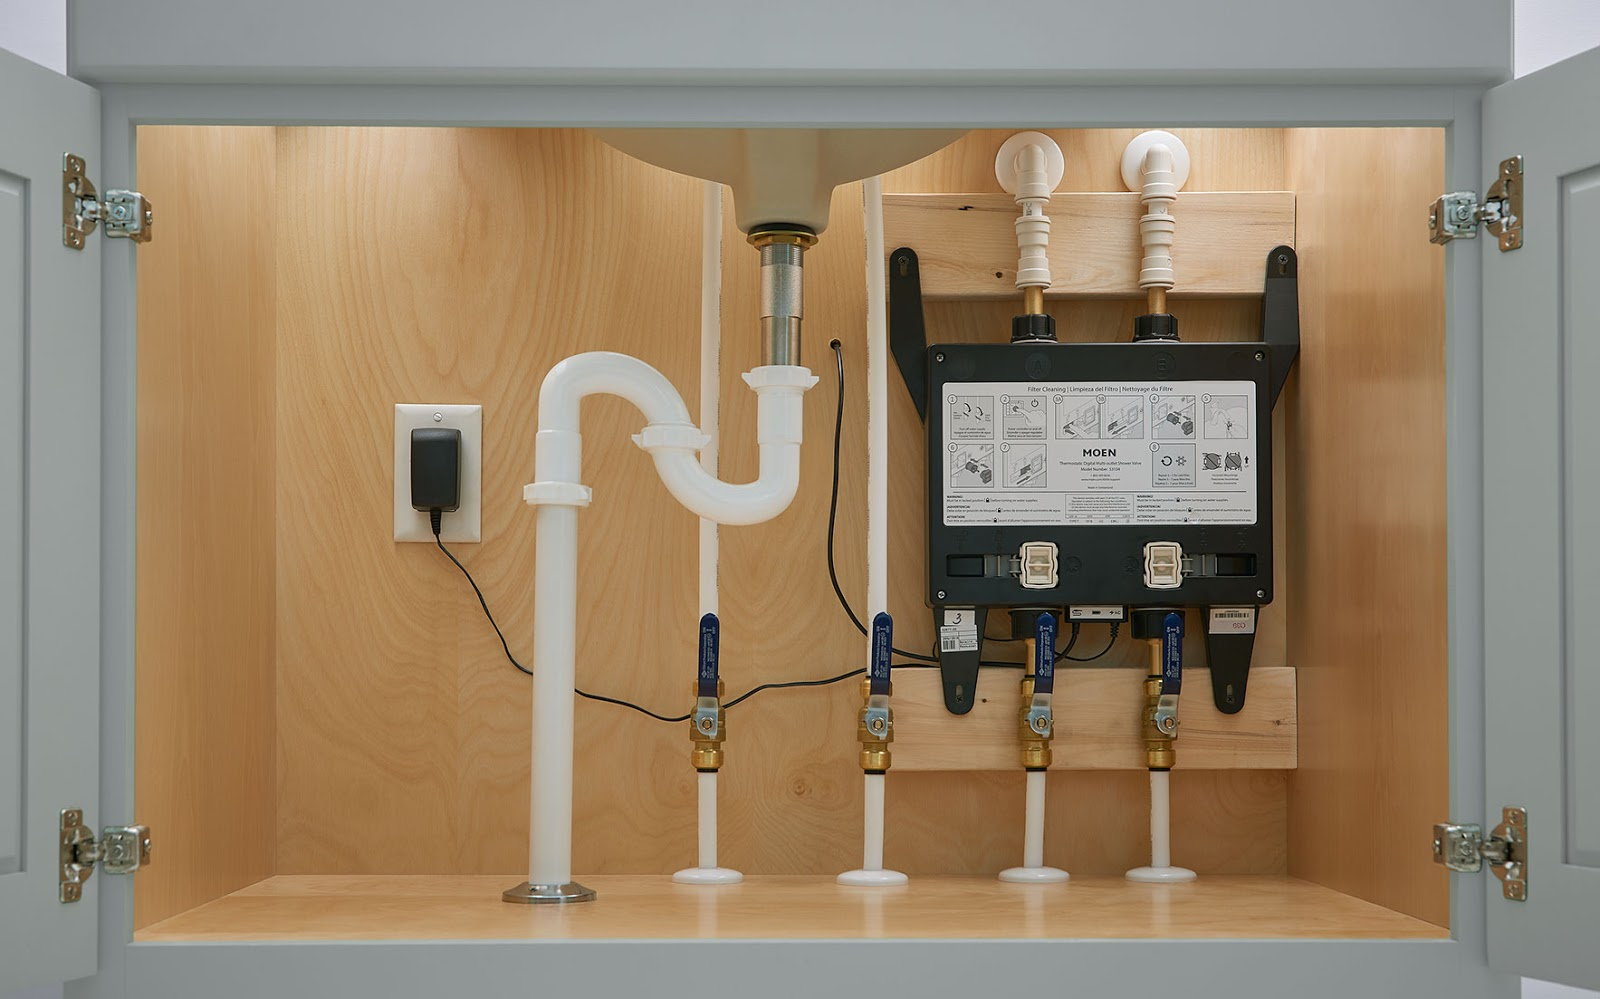
\includegraphics[width=0.8\linewidth]{img/under-cabinet-valve.jpg}
                        \caption{U by Moen digital valve}
                    \end{figure}
            \subsubsection{Livin\cite{livin}}
                \paragraph{}
                    Much like the previously mentioned U by Moen showers in terms of ‘smart’ functions. Showers preparation, 
                    temperature, duration and different shower profile settings can be controlled and monitored via an app or 
                    voice control (Amazon Alexa or Google Home). Some added features include music control (requires external 
                    speaker) using the shower digital controller. The company claims that the system is easy to install with 
                    simple hand tools and it can be retrofitted with most single-handle valve types on the market. The entire 
                    system is powered by a  detachable and rechargeable battery unit that is able to last up to 2 months with 
                    normal use, according to the company. In case the battery run out, the shower can still be controlled with 
                    the manual handle.
                \paragraph{}
                    Product package includes valve, shower head, mounting plate, adapter, battery and charging dock for the battery. 
                    The shower system costs \$599 USD. However as of May 2019, the product is not yet brought to the market despite 
                    its initial plan being in Fall 2018 due to financial problems.
                    \begin{figure}[H]
                        \centering
                        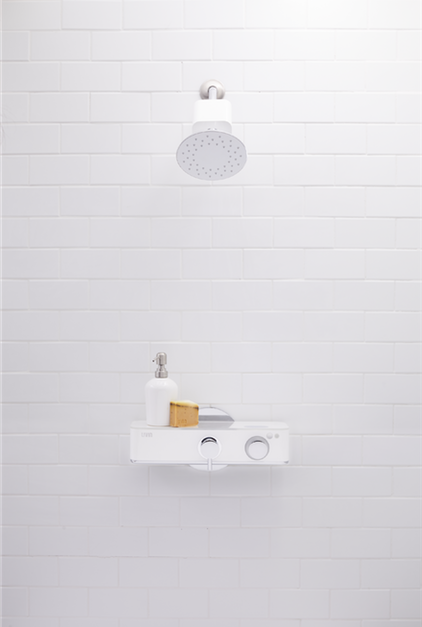
\includegraphics[width=0.4\linewidth]{img/LivinPhoto.png}
                        \caption{Livin smart shower}
                    \end{figure}
        \subsection{Product Advantages and Disadvantages}
            \paragraph{}
                The main advantage of our system is that it is adding value to an existing product to further enhance its capabilities. This is achieved through 
                the inclusion of an advanced user interface. Our product may also provide retrofitting capability dependant upon our energy generation tests.
            \paragraph{}
                One disadvantage of our smart shower system is compatibility only with double-handle type valves ie. separate hot and cold inlets to the system. 
                This can be resolved with modifications post-production.
        \subsection{Marketing Strategy}
            Since our product is integrated with Enware’s existing system, our marketing strategy is based around adding value to an existing solution. As there 
            are not many smart shower systems on the market, the product will be able to cement a foothold in an emerging sector. This will be achieved in 
            collaboration with Enware.

    \newpage
    \section{Product Design}
        \subsection{Hardware}
            \subsubsection{Overview}
                \paragraph{}
                    Daedal is focused on researching and developing the possibilities of thermoelectric and hydroelectric generation as the current 
                    system is directly supplied from the electrical grid. Daedal’s approach is to create a system using the energy produced through 
                    showering, and to explore if it is feasible to internally supply the system. This is to be achieved through thermoelectric generation, 
                    using the temperature difference between the inlet and outlet as well as using the moving water to create hydroelectric generation.
            \subsubsection{Background}
                \subsubsubsection{Thermoelectric Generator}
                    \paragraph{}
                        Thermoelectric generators are a solid state device that operates on the principle known as the Seebeck effect. The Seebeck effect 
                        defines that a voltage is produced between two different conductive materials when there is a temperature difference between them
                        \cite{thermoelectricity}. The greater the temperature difference between the conductors, the greater the voltage. If a load is 
                        connected between the terminals, a direct current will flow. Thermoelectric generators have the unique property, that when a voltage 
                        is applied (rather than produced) to the terminals, a temperature difference is setup across the device. Additionally, swapping the 
                        polarity on the device will also swap the temperature difference on the materials (heat side will become the cool side).
                    \paragraph{}
                        The generated voltage follows the equation:
                        \[\Delta V = S_{ab} (T_h - T_c)\]
                    \paragraph{}
                        $S_{ab}$ is the Seebeck coefficient measured in V/K between two materials. The Seebeck coefficient is also dependant on temperature 
                        which results in an optimal temperature for the junctions to be at.  When operating at this temperature, maximum power is achieved. 
                        $T_h$ is the hot side temperature and $T_c$ is the cold side temperature. 
                    \paragraph{}
                        A key design challenge when using thermoelectric generators is to minimise heat conduction from one side of the device to the other. 
                        If this occurs, the temperature difference between sides is reduced which results in lower output voltage.
                \subsubsubsection{Hydroelectric Generator}
                    \paragraph{}
                        Hydroelectric generators have a turbine which are connected to an electrical generator. If the turbine is rotated, so is the generator 
                        which in-turn generates electricity. The amount of power produced can be related by the following equation\cite{pump_power}. 
                        \[P=\frac{\rho gH_l}{\eta}\]
                        where:\\
                        \indent P = Power (watts)\\
                        \indent $\eta$ = Efficiency\\
                        \indent $\rho$ = Density (water  = 1000 kg/$m^3$)\\
                        \indent g = gravity (m/$s^2$)\\
                        \indent $H_l$ = head loss (m), amount of fluid pressure over a distance
                    \paragraph{}
                        Through the understanding of fluid mechanics the properties can be explored and calculations done to understand the losses and generation 
                        occuring during operation.
                    \paragraph{}
                        Turbines can have multiple designs each of which have benefits and drawbacks. Turbines similar to a water wheel are simple but large. 
                        Alternatively, axial turbines similar to jet engines are small but more complicated to manufacture.
                    \paragraph{}
                        A key design challenge when using turbines for such uses are, to minimise pressure loss across turbine while extracting the ideal amount 
                        of power.
            \subsubsection{Design of Test Layout}
                \paragraph{}
                    The initial design for the research and development of a self generating system is simple with easy access to each generation source. Due to 
                    the nature of electricity and water, it is important to isolate these properly. This can be achieved by following industry standards. The 
                    design is set up to be able to individually test each generation. The test layout will also measure the temperature and pressure of the system, 
                    with different configurations, to validate what would both produce the best electrical generation and comfort of the user.
                \paragraph{}
                    If results are found, that it is feasible to make the system independent of the electrical grid. A redesign of the layout and addition of a 
                    battery system will be added.
                    \begin{figure}[H]
                        \centering
                        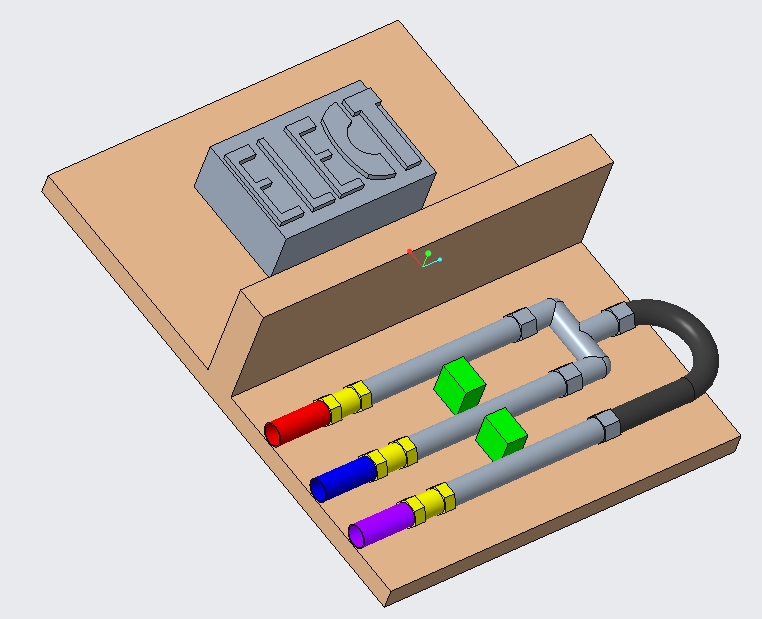
\includegraphics[width=0.8\linewidth]{img/testingSetup.png}
                        \caption{CAD model of Testing System}
                    \end{figure}
            \subsubsection{Electrical Schematics}
                \paragraph{}
                    The electrical layout for the test layout is designed with modularity as the key requirement. Each generator will have its set of electrical 
                    connections running to banana plugs. A wattmeter and load resistor will also be mounted onto the test layout with connections running to banana 
                    plugs also. Figure 4 displays the connection layout.
                    \begin{figure}[H]
                        \centering
                        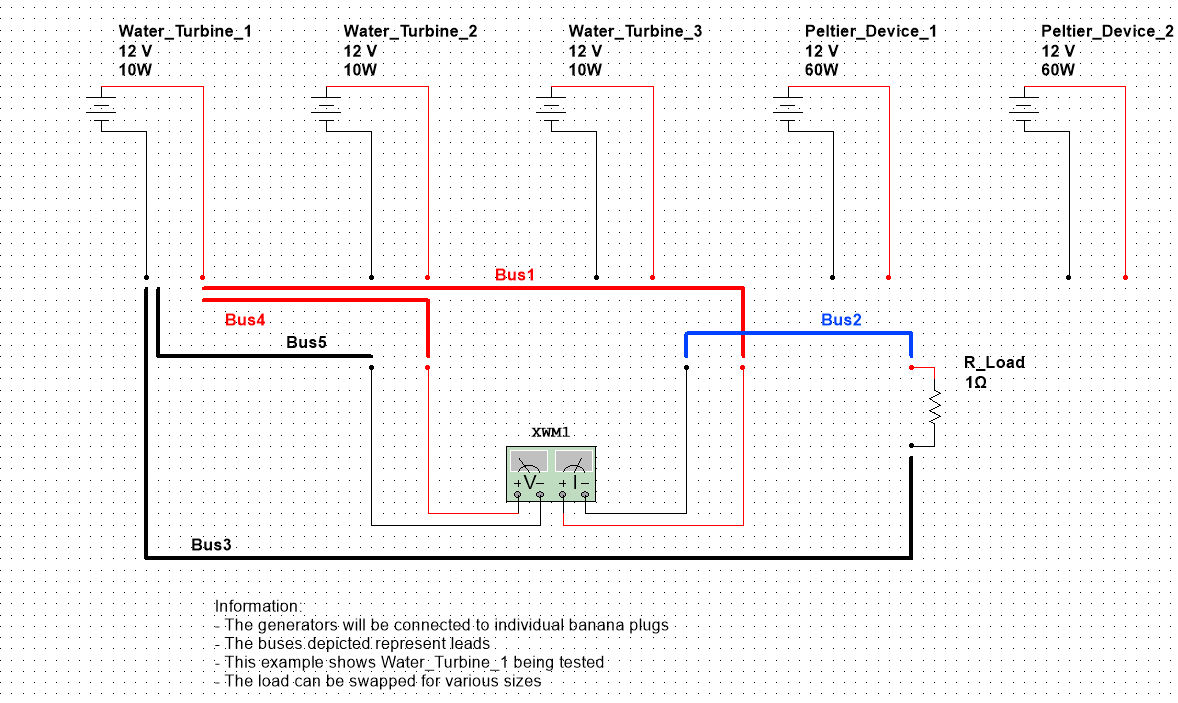
\includegraphics[width=0.8\linewidth]{img/circuitDiagram1.png}
                        \caption{Test layout electrical schematic}
                    \end{figure}
            \subsubsection{Testing Procedures}
                \paragraph{}
                    As described in the design, multiple elements need to  be tested, recorded and reviewed to determine if it is feasible to remove the system 
                    from the electrical grid. The results needed are current, voltage and power of both the hydroelectric and thermoelectric generators, as well 
                    as volumetric flow rate of the inlet and outlet pipes. The recording of the electrical equipment will determine if the generated electricity 
                    is enough to power the system, where as the measuring of the flow rate can determine how much pressure is lost to the system and if that 
                    impacts the users experience.
                \paragraph{}
                    To create the best overview of success in the research and development is to repeat the tests over each scenario to determine what is going 
                    to create the most electricity while not impacting the experience of the user. These scenarios are:
                    \spacing{1}
                    \begin{itemize}
                        \item No generators - comparing result
                        \item 1 inlet pipe turbine generator
                        \item 2 inlet pipe turbine generators
                        \item 2 inlet pipe and 1 outlet pipe turbine generators
                        \item 1 outlet turbine generator
                        \item Thermoelectric generation between hot and cold inlet pipes
                        \item Thermoelectric generation between cold inlet and mixed outlet pipe
                        \item Both scenarios of thermoelectric generation above
                        \item 2 inlet and 1 outlet turbine generators and both thermoelectric generators
                    \end{itemize}
                \spacing{1.5}
                \paragraph{}
                    From this collected data, Daedal will be able to completely determine the feasibility of removing the system from the electrical grid by either 
                    adding or removing more generators.
                \paragraph{}
                    Below is an example of how the electrical side of the test layout will be connected during testing. Figure 5 depicts water turbine 1 being tested.
                    \begin{figure}[H]
                        \centering
                        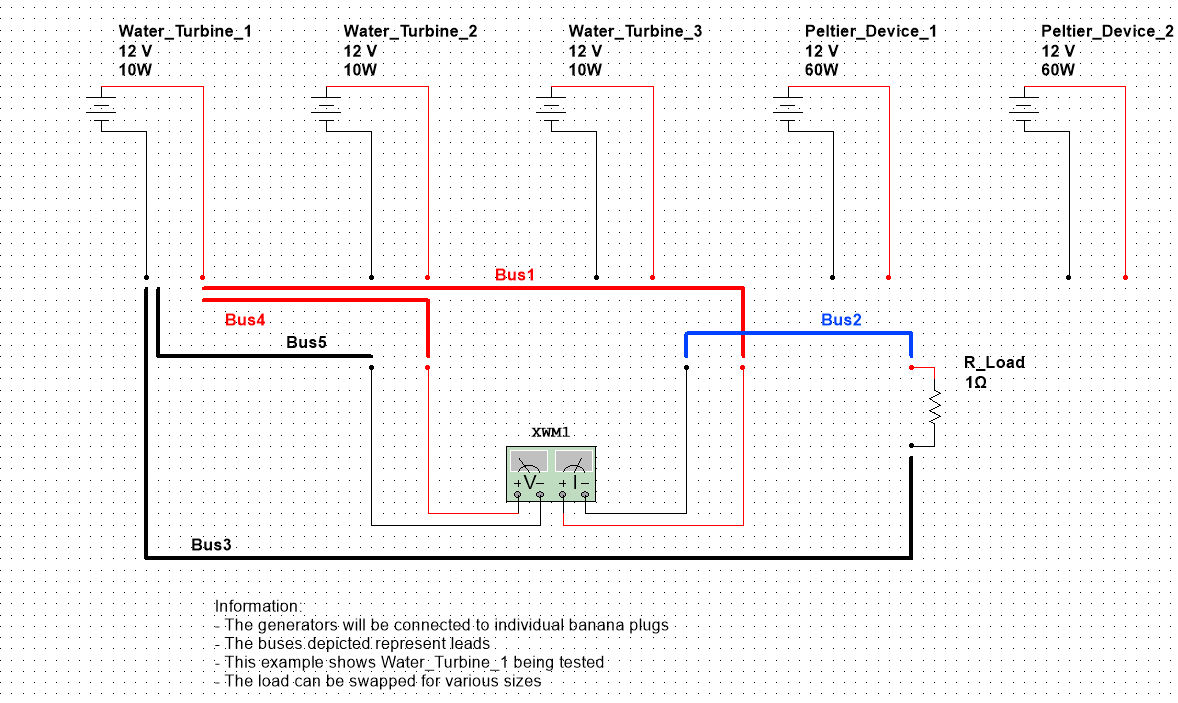
\includegraphics[width=0.8\linewidth]{img/circuitDiagram2.png}
                        \caption{Wiring of test layout for testing water turbine 1}
                    \end{figure}
            \subsubsection{Expected Outcomes}
                \paragraph{}
                    During our testing we expect electricity to be generated.  However, the exact amount generated, as well as pressure lost in the shower system 
                    is unknown. Daedal is predicting the designs above may produce enough  to make the system completely independent of the electrical grid. 
                    Dependent of results, Daedal will aim to create a solution for making the system completely or partially independent of the electrical grid 
                    creating a more sustainable product.
        \newpage
        \subsection{Software}
            \subsubsection{Overview}
                \paragraph{}
                    The software for the web interface of our smart shower is designed to be easily used by anyone wishing to control the shower whilst ensuring 
                    the safety and privacy of our users. Our software solutions include native compatibility with all aspects of our hardware solutions, long 
                    term storage and analysis of showering data for many users using the smart shower system. Additionally our software solution will provide 
                    secure administrative control over both users and devices to ensure safe and easy operation for users of all age levels.
            \subsubsection{Server Setup}
                \paragraph{}
                    The Raspberry Pi will collect the data, store it and provide a means to observe the data by running a locally hosted server. To do this the 
                    Raspberry Pi will run the Raspbian Stretch Lite Operation System from the Raspberry Pi Foundation\cite{raspbian}. Installed on this system 
                    will be Node Package Manager, Node.js and MySQL to form the core of our data storage and server setup. These will be installed via the command 
                    line using the following commands:
                    \footnotesize
                    \spacing{1}
                    \begin{figure}[H]
                        \begin{lstlisting}
    > sudo apt-get update
    > sudo apt-get upgrade
    > wget 
      https://nodejs.org/dist/v10.15.3/node-v10.15.3-linux-armv6l.tar.xz
    > tar -xzf node-v10.15.3-linux-armv6l.tar.gz
    > cd node-v6.11.1-linux-armv6l/
    > sudo cp -R * /usr/local/
    > npm install mysql
                        \end{lstlisting}
                        \caption{Environment Install Bash Commands}
                    \end{figure}
                \normalsize
                \spacing{1.5}
                \paragraph{}
                    Once that is completed the server can be run using a javascript file that handles both the http connection and the database side of the server.
                \paragraph{}
                    The database will consist of two parts, a MySQL server storing the information (Contact Details, Settings, Preferences, Restrictions, etc.) 
                    of the users and the devices, in this format:
                    \begin{figure}[H]
                        \centering
                        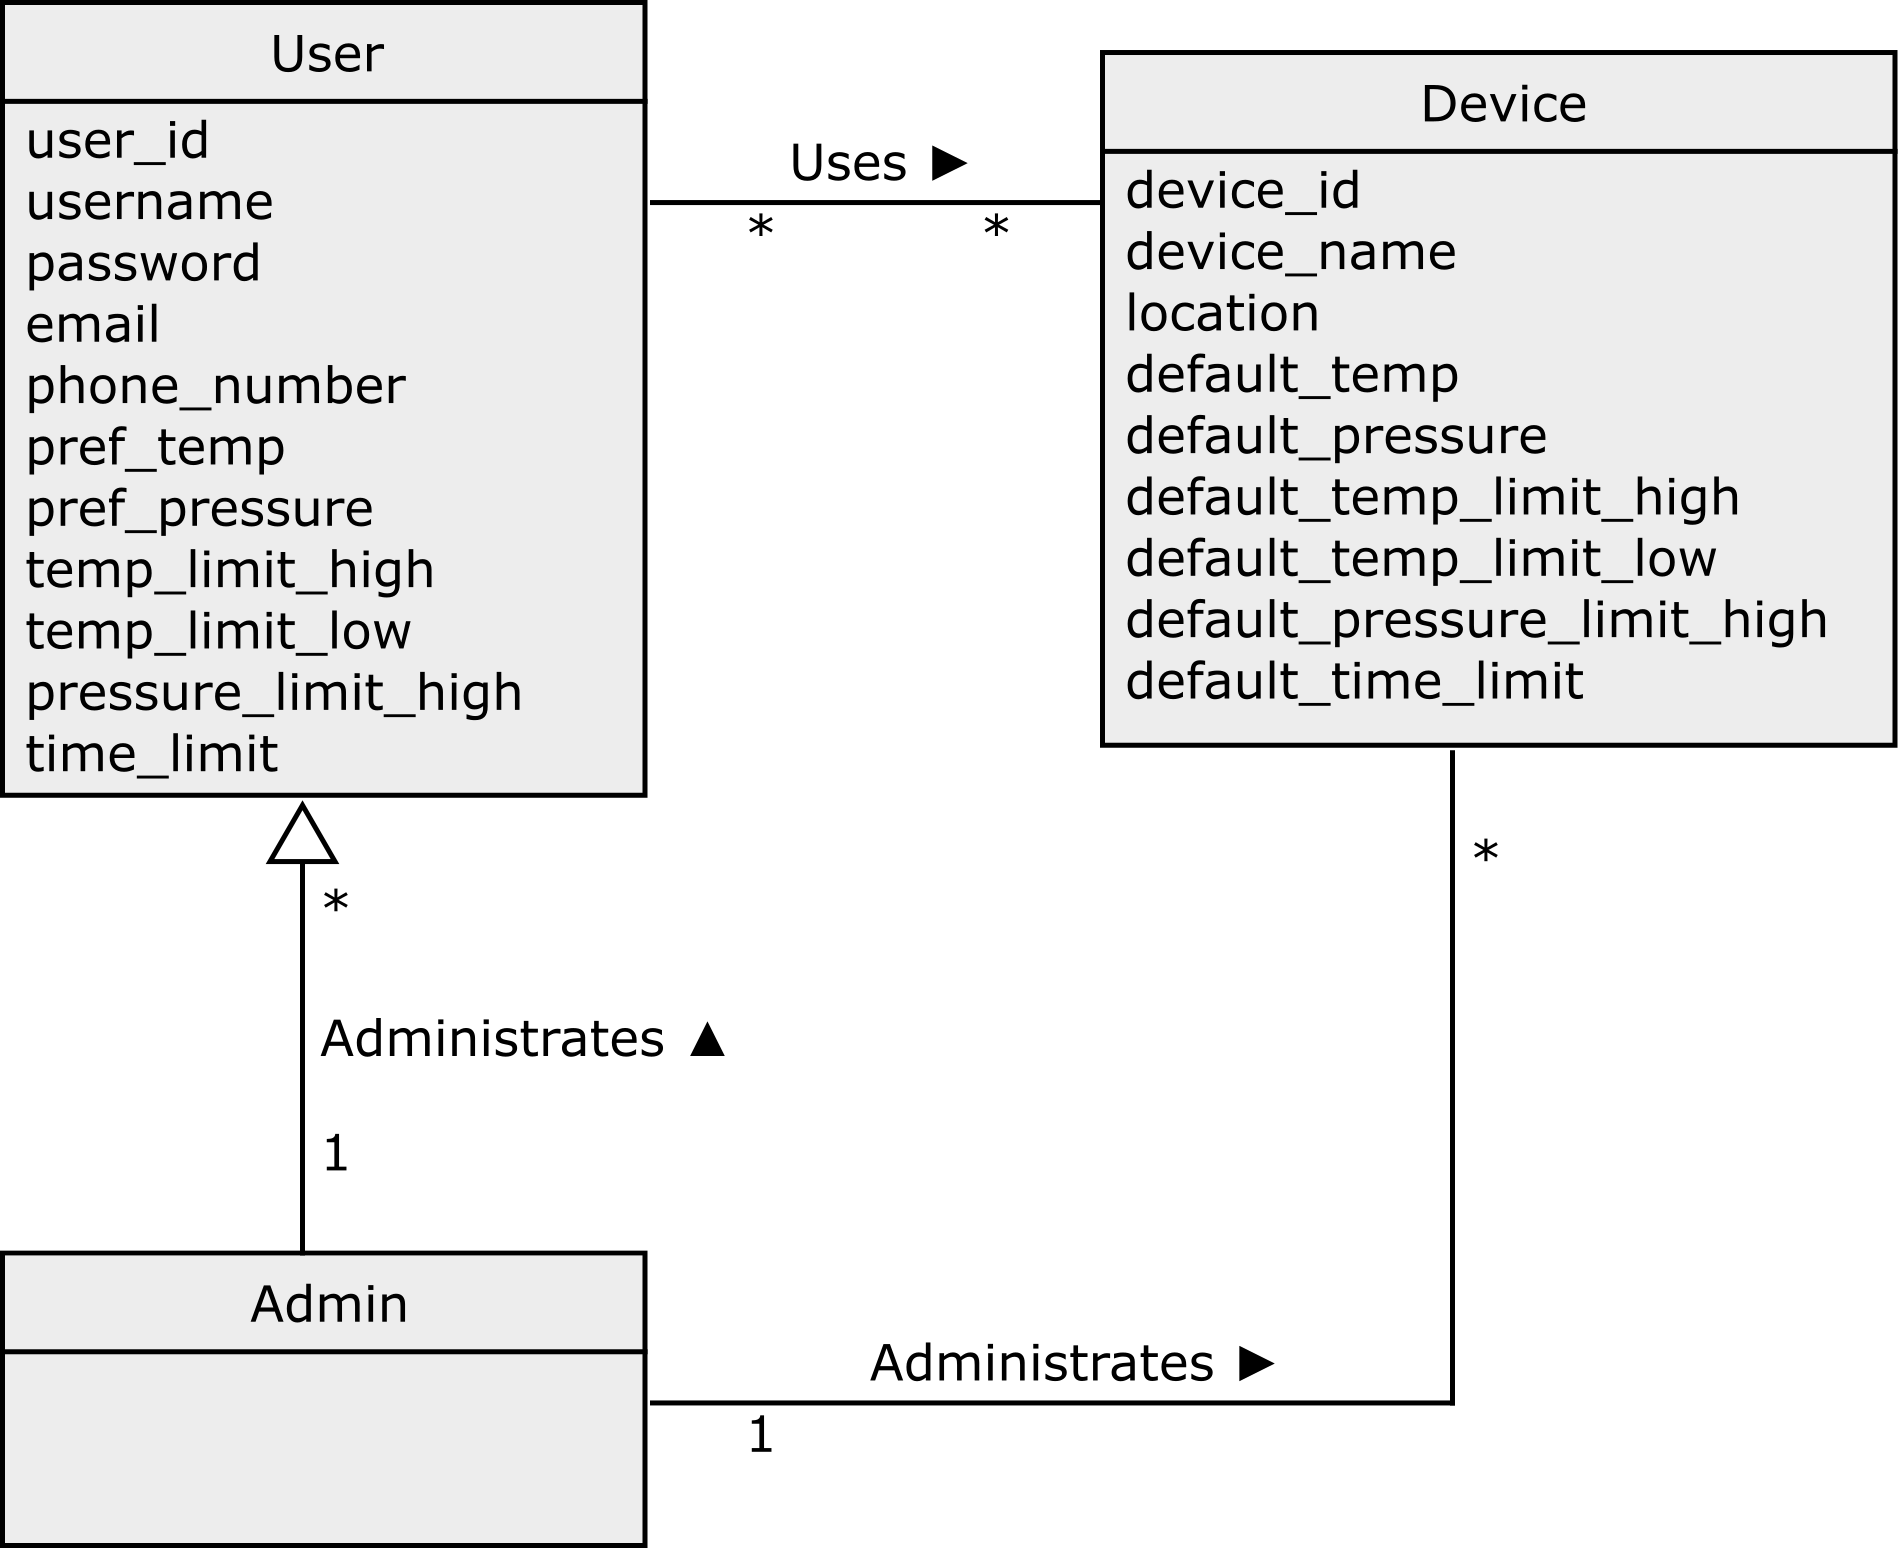
\includegraphics[width=0.8\linewidth]{img/SettingsDatabaseUML_large.png}
                        \caption{Settings Database UML Diagram}
                    \end{figure}
                \paragraph{}
                    The second part will be a JSON-based database holding the data logged from the device, so that we can analyse this data and present it in a 
                    human readable format. We will also attempt to set up an api for accessing the raw data, via the http server. The JSON-database will have the 
                    following structure:
                    \footnotesize
                    \spacing{1}
                    \begin{figure}[H]
                        \begin{lstlisting}
    {
        "$device_id": "????????????????",
        "connections": [
            {
                "start_time": ##########,
                "end_time": ##########,
                "$user_id": "????????????????",
                "data": [
                    {
                        "timestamp": ##########,
                        "temp": ##.#,
                        "pressure": ##.##
                    }, ...
                ]
            }, ...
        ]
    }
                        \end{lstlisting}
                        \caption{Data Database JSON Structure}
                    \end{figure}
                \normalsize
                \spacing{1.5}
                \paragraph{}
                    A javascript file will both manage the database connections as well as the setup and connections to the http server. So that the device may 
                    be controlled from anywhere on the local network. If an internet connection is unknown or not available the Raspberry Pi will automatically 
                    create a WiFi hotspot prompting anyone that connects to it to input WiFi credentials for one of the detected available networks. This javascript 
                    document will have the following structure:
                    \footnotesize
                    \spacing{1}
                    \begin{figure}[H]
                        \begin{lstlisting}
    import required packages
    setup global variables
    function checkInternetConnection() {
        Check for  available internet connections
        Check if available internet connections are known
        if known connect
        else
            create wifi hotspot
            prompt for internet login details
            update known internet connections
            Connect
    }
    function SetupMySQLDatabase() {}
    function ConnectToMySQLDatabase() {}
    function CreateHTTPServer() {
        Listen for connections
        Get requested data
        Write requested data
        Loop
    }
                        \end{lstlisting}
                        \caption{Server Setup and Management File}
                    \end{figure}
                \normalsize
                \spacing{1.5}
            \subsubsection{Interface Design}
                \paragraph{}
                    The goal for the design of the interface is to create an environment which is easy to use, taking into consideration elderly people who 
                    are losing their physical dexterity. To achieve this we have decided to create a web interface which focuses on making the buttons large, 
                    clear and easy to use. Additionally, the layout has been designed in order to maximise the visibility of the most critical information. 
                    This is showcased in the following mockup:
                    \begin{figure}[H]
                        \centering
                        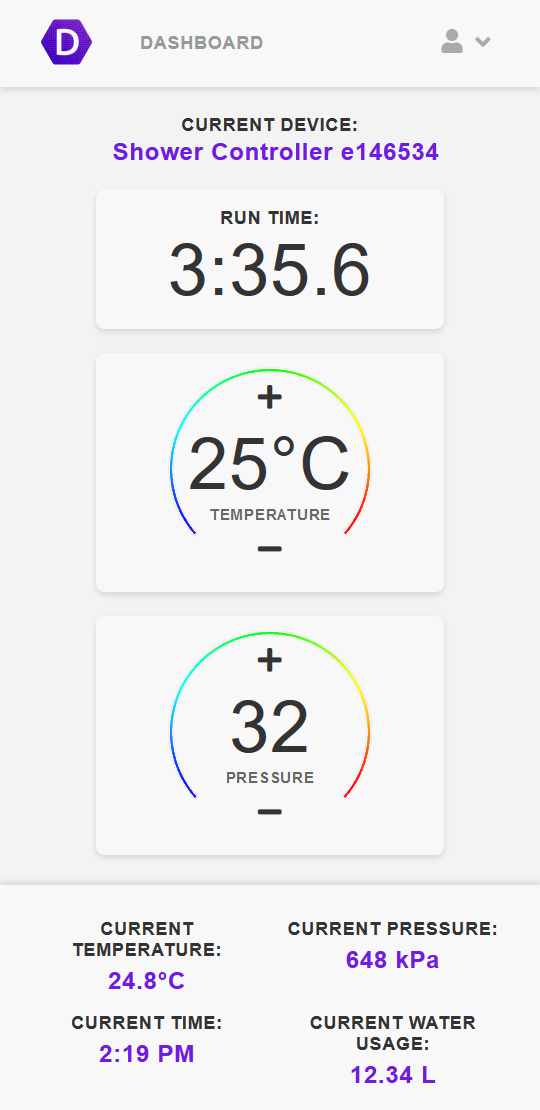
\includegraphics[width=0.5\linewidth]{img/Daedal_Mobile1.png}
                        \caption{Mobile Interface Mockup}
                    \end{figure}
                \paragraph{}
                    Our interface design also aims to be flexible so that it works and achieves its goals on many devices and screen sizes. To do this we have 
                    designed the web interface to adapt to the size of the screen. You can see an example of a larger screen size below in Figure 11.
                    \begin{figure}[H]
                        \centering
                        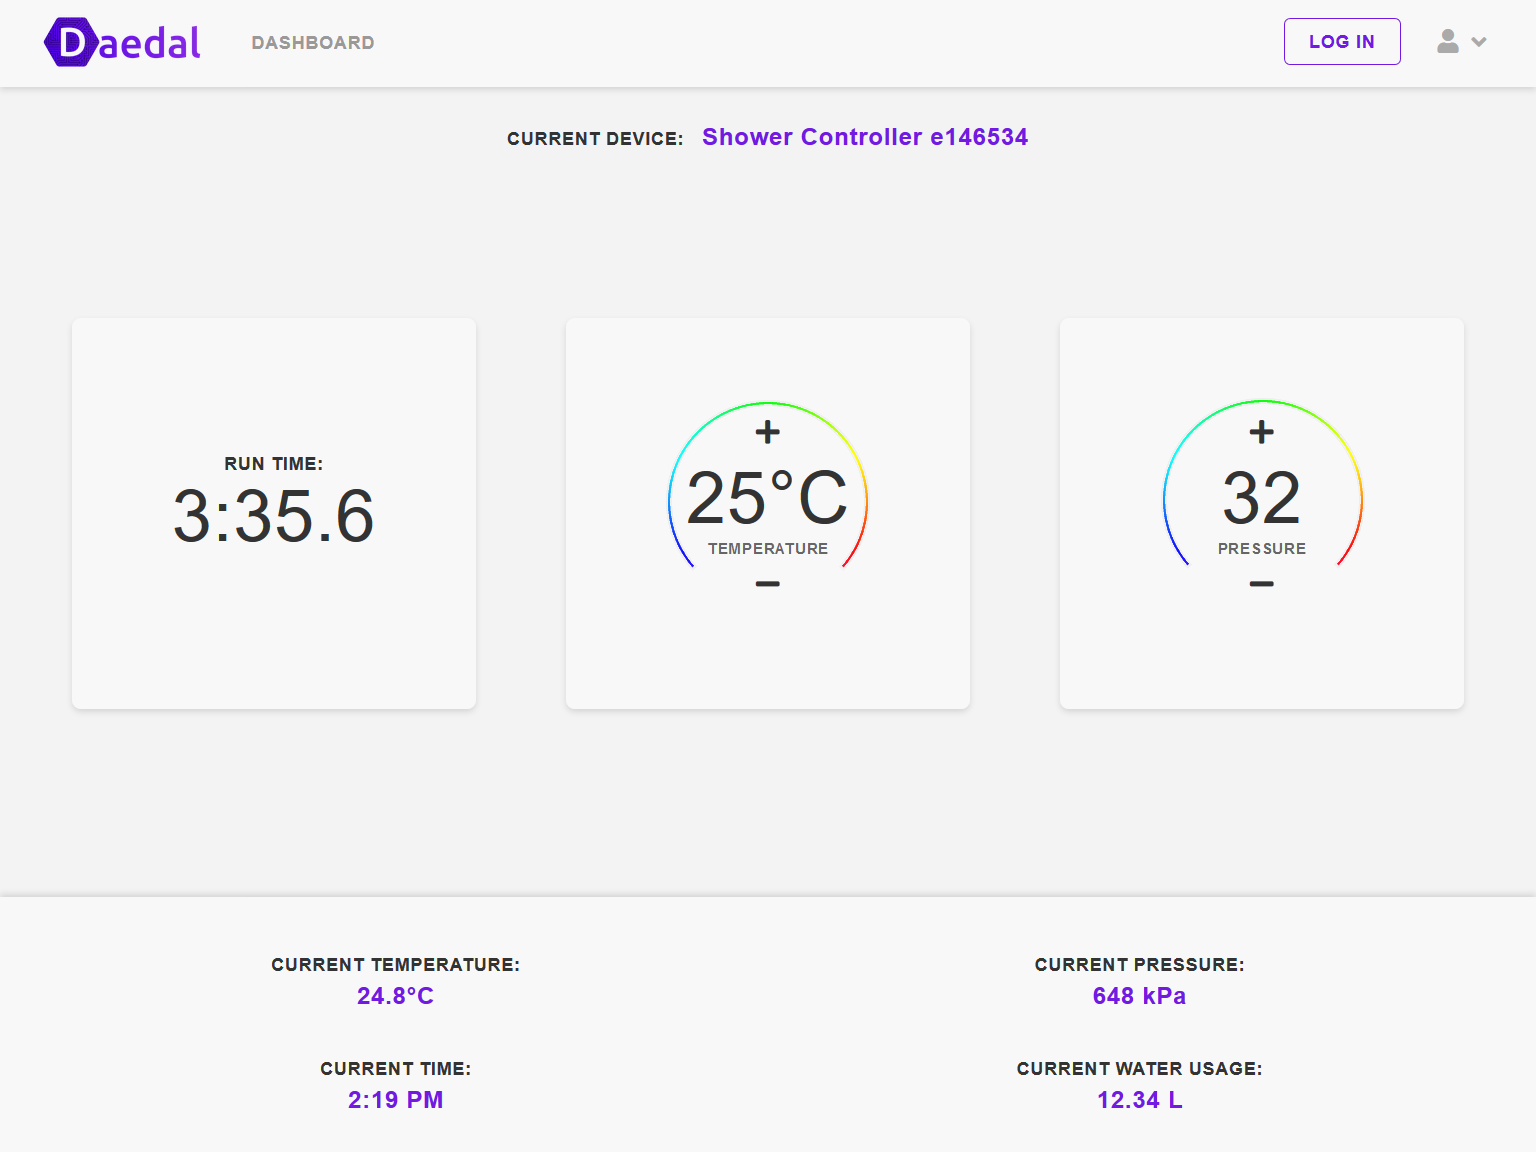
\includegraphics[width=0.8\linewidth]{img/Deadal_Tablet1.png}
                        \caption{Tablet/Desktop Interface Mockup}
                    \end{figure}
                \paragraph{}
                    The final purpose of our web interface is to display the data taken from the shower system in various formats, providing a means for administrators 
                    to control the devices and users they manage. The interface for these controls can be seen below in Figure 12.
                    \begin{figure}[H]
                        \centering
                        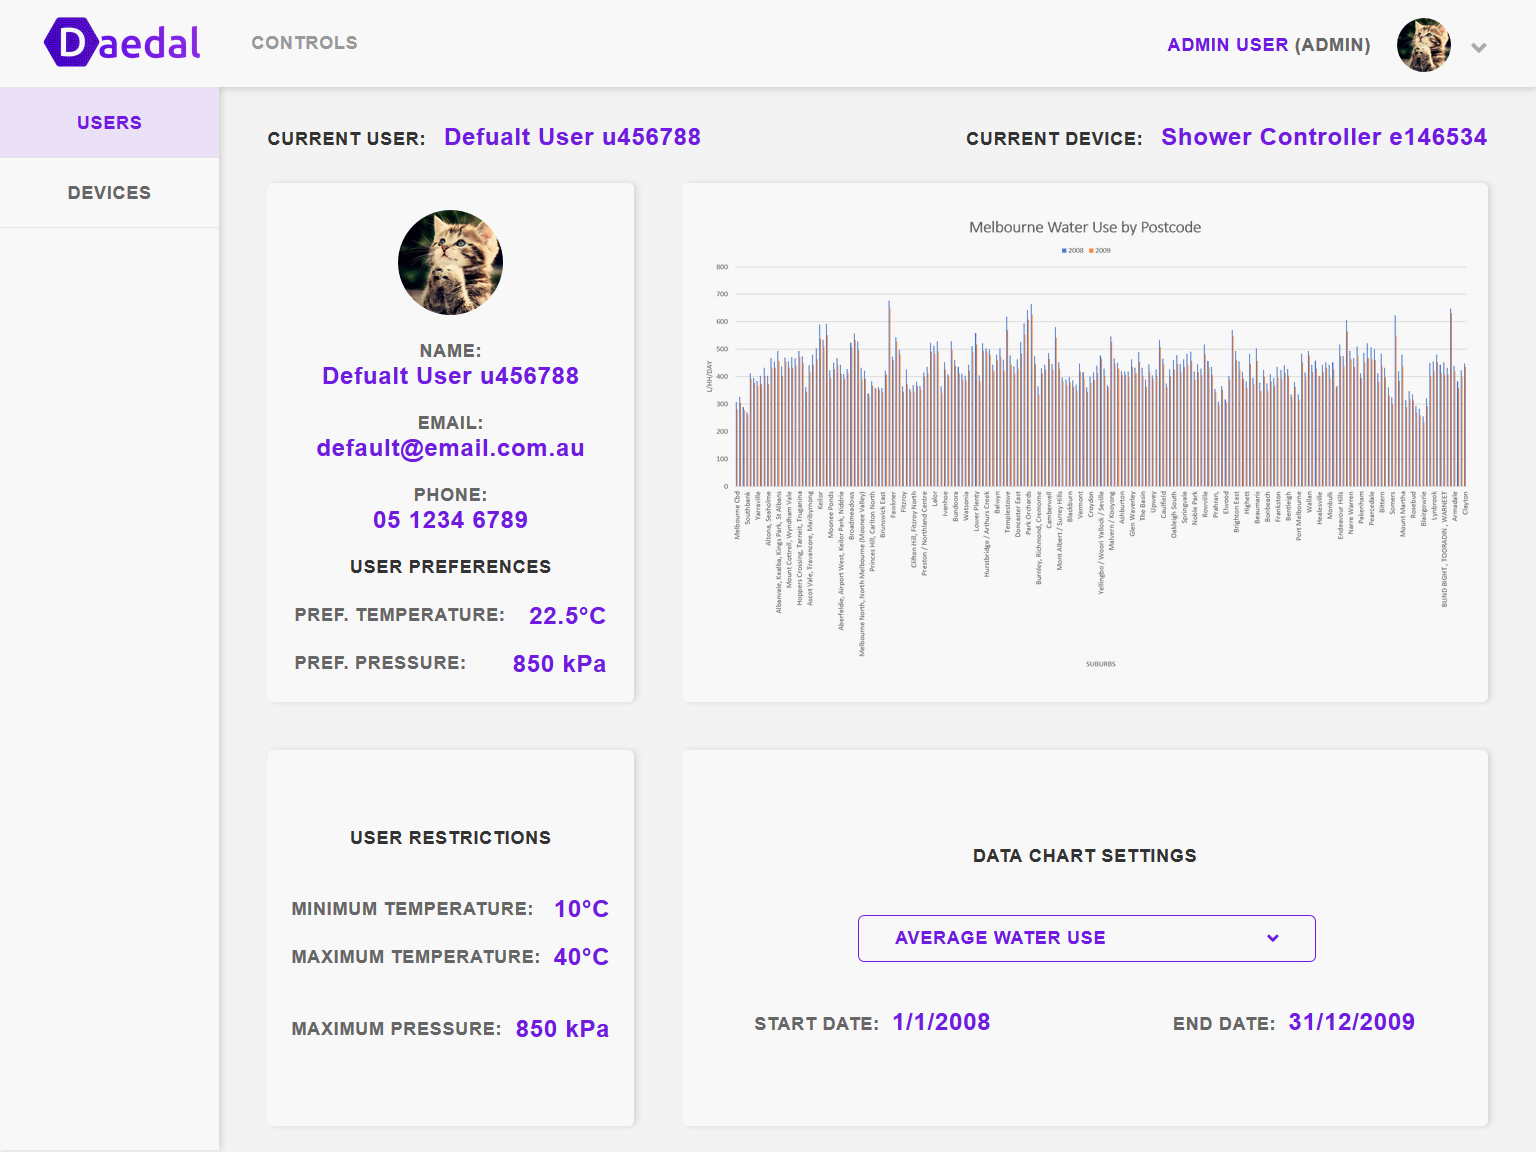
\includegraphics[width=0.8\linewidth]{img/Tablet_Data_Interface1.png}
                        \caption{Tablet/Desktop Data and Admin Interface Mockup}
                    \end{figure}
                \paragraph{}
                    When a user seeks to view the above page they must first be logged on. They can do this by entering their details into a form accessed through 
                    the “Login” button or the settings dropdown on the main screen.
                    \begin{figure}[H]
                        \centering
                        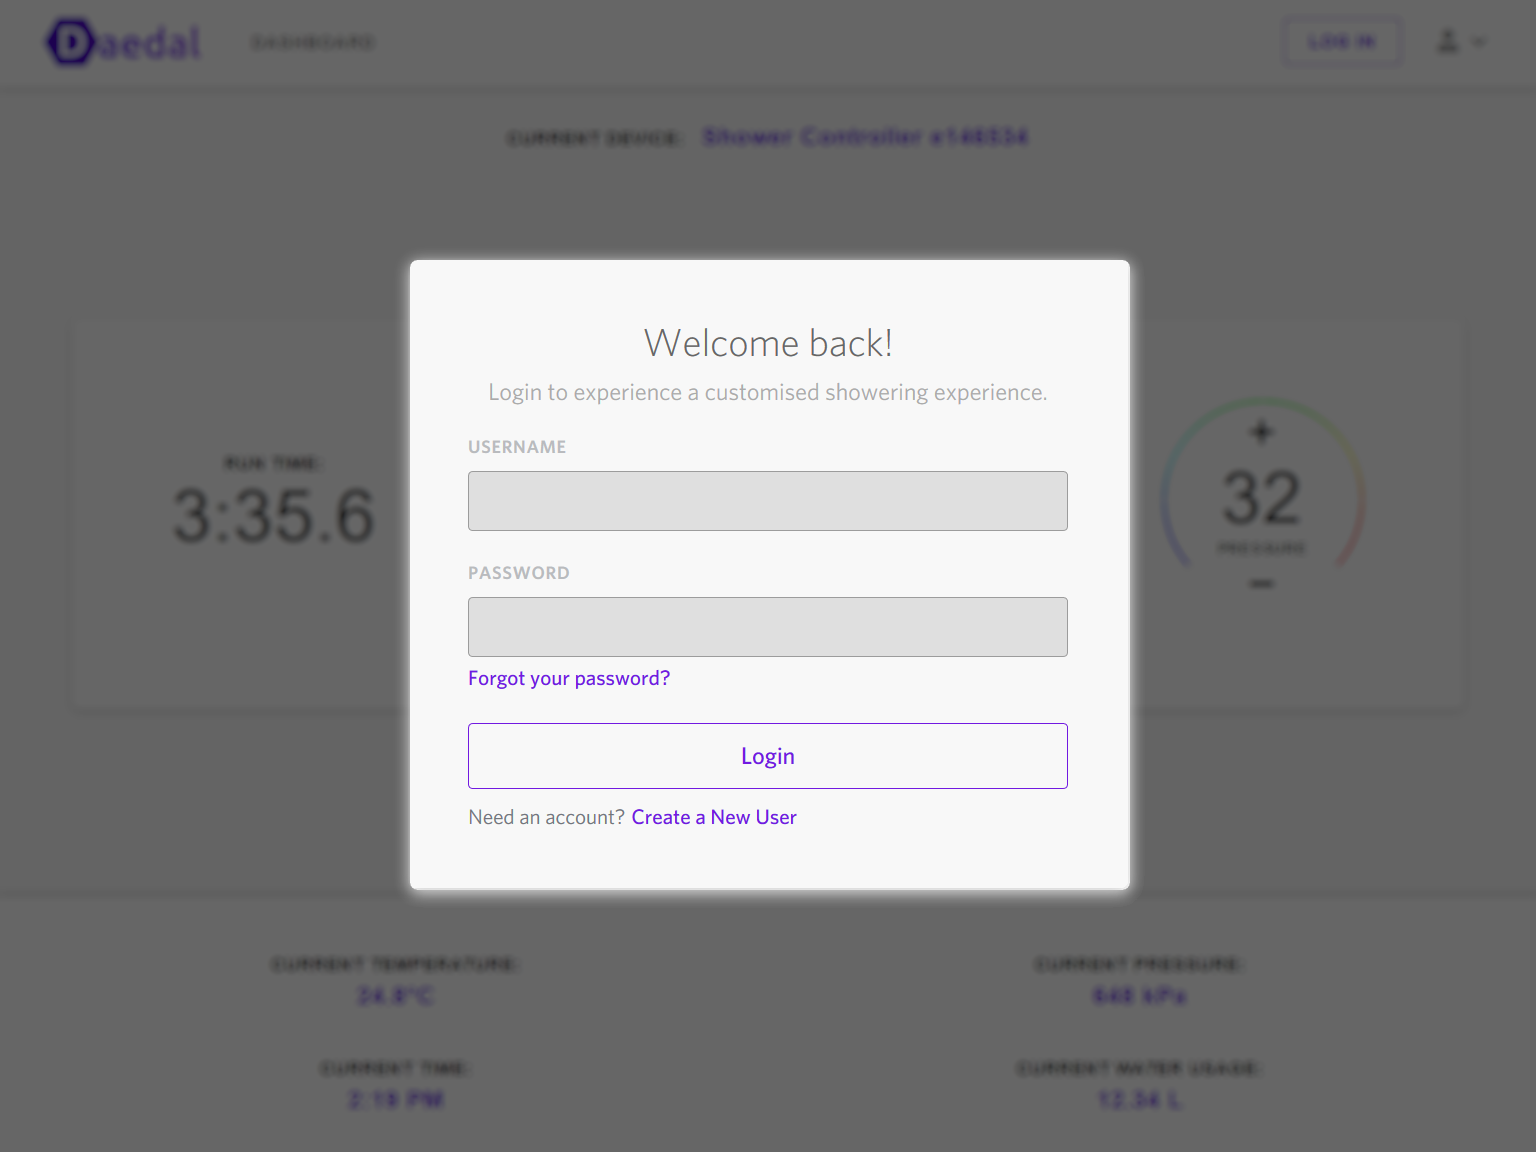
\includegraphics[width=0.8\linewidth]{img/Deadal_Tablet2.png}
                        \caption{Login Interface Mockup}
                    \end{figure}
            \subsubsection{Interface Functions}
                \paragraph{}
                    \begingroup
                        \centering
                        \begin{flushleft}
                            \resizebox{\linewidth}{!} {
                                \begin{tabular}{| m{0.4\linewidth} | m{0.6\linewidth} |}
                                    \hline
                                    \textbf {Fields} & \textbf {Functions} \\ \hline
                                    Username & Drops down to show list of users  \\ \hline
                                    Password & Allows to enter password  \\ \hline
                                    Login & Interfaces to respective admin/user  \\ \hline
                                    Create a new user & Interfaces to new user setup page  \\
                                    \hline
                                \end{tabular}
                            }
                            \captionof{table}{LogIn interface fields}\label{tbl:LogIntable}
                        \end{flushleft}
                    \endgroup
                    \footnotesize
                    \spacing{1}
                    \begin{figure}[H]
                        \begin{lstlisting}
    function LogInButtonClicked() {
        Get the username
        Get the password
        Hash the password
        Send the username and password hash to the server
        if (the username and password matches a user) {
            Login
        } else {
            Display Error
            Clear the login form
            Prompt the user to reattempt the login form
        }
    }                        
                        \end{lstlisting}
                        \caption{Function for when the LogIn Button is clicked}
                    \end{figure}
                    \normalsize
                    \spacing{1.5}
                \paragraph{}
                    \begingroup
                        \centering
                        \begin{flushleft}
                            \resizebox{\linewidth}{!} {
                                \begin{tabular}{| m{0.4\linewidth} | m{0.6\linewidth} |}
                                    \hline
                                    \textbf {Fields} & \textbf {Functions} \\ \hline
                                    Users & Displays a list of all users controlled by admin  \\ \hline
                                    Devices & Displays a list of all devices controlled by admin  \\ \hline
                                    Minimum Temperature User Restriction & Sets the lower limit the temperature can be set to  \\ \hline
                                    Maximum Temperature User Restriction & Sets the upper limit the temperature can be set to  \\ \hline
                                    Maximum Pressure User Restriction & Sets the upper limit the pressure can be set to  \\ \hline
                                    Data Chart Settings Dropdown & Select what data to display in the chart \\ \hline
                                    Data Chart Settings Start Date & Set the start date for the data displayed in the chart  \\ \hline
                                    Data Chart Settings End Date & Set the end date for the data displayed in the chart  \\
                                    \hline
                                \end{tabular}
                            }
                            \captionof{table}{User Restrictions interface fields}\label{tbl:userrestrictionstable}
                        \end{flushleft}
                    \endgroup
                    \footnotesize
                    \spacing{1}
                    \begin{figure}[H]
                        \begin{lstlisting}
    function UpdateDataChart() {
        Get start date
        Get end date
        Get result of data chart dropdown
        function RetrieveDataFromDatabase() {}
        function PerformOperationsOnData() {}
        function DisplayDataInChart() {}
    }                                              
                        \end{lstlisting}
                        \caption{Function for updating the data chart}
                    \end{figure}
                    \normalsize
                    \spacing{1.5}
                    \footnotesize
                    \spacing{1}
                    \begin{figure}[H]
                        \begin{lstlisting}
    function SetUserRestrictions() {
        Get Minimum Temperature User Restriction
        Get Maximum Temperature User Restriction
        Get Maximum Pressure User Restriction
        function WriteRestrictionsToDatabase() {}
    }                                                                     
                        \end{lstlisting}
                        \caption{Function for setting the user restrictions}
                    \end{figure}
                    \normalsize
                    \spacing{1.5}
                \paragraph{}
                    \begingroup
                        \centering
                        \begin{flushleft}
                            \resizebox{\linewidth}{!} {
                                \begin{tabular}{| m{0.4\linewidth} | m{0.6\linewidth} |}
                                    \hline
                                    \textbf {Fields} & \textbf {Functions} \\ \hline
                                    Display Set Temperature & Displays the set temperature preference for user  \\ \hline
                                    Display Set Pressure & Displays the set pressure preference for user  \\ \hline
                                    Increment Set Temperature & Increments the set temperature preference for user  \\ \hline
                                    Decrement Set Temperature & Decrements the set temperature preference for user  \\ \hline
                                    Increment Set Pressure & Increments the set pressure preference for user  \\ \hline
                                    Decrement Set Pressure & Decrements the set pressure preference for user \\ \hline
                                    Display Current Run Time & Displays how long the shower has been running for  \\ \hline
                                    Display Current Temperature & Displays the current temperature of the shower  \\ \hline
                                    Display Current Clock Time & Displays the current 12/24 hour clock time  \\ \hline
                                    Display Current Pressure & Displays the current pressure of the shower  \\ \hline
                                    Display Current Total Water Usage & Displays the total amount of water used this sessionn  \\
                                    \hline
                                \end{tabular}
                            }
                            \captionof{table}{Main page user interface fields}\label{tbl:userinterfacetable}
                        \end{flushleft}
                    \endgroup
                    \footnotesize
                    \spacing{1}
                    \begin{figure}[H]
                        \begin{lstlisting}
    function ChangeTemperature/Pressure() {
        Detect Changes to Temperature or Pressure
        if (input less than or greater than control limits set by admin) {
            Display error
        } else {
            Write Temperature or Pressure to hardware
            Write Temperature or Pressure changes to database
        }
    }                                                                
                        \end{lstlisting}
                        \caption{Function for the Temperature or Pressure}
                    \end{figure}
                    \normalsize
                    \spacing{1.5}
                    \footnotesize
                    \spacing{1}
                    \begin{figure}[H]
                        \begin{lstlisting}
    Loop once a second {
        Get current temperature
        Display current temperature
        Get the current time
        Display the current time
        Get current pressure
        Display current pressure
        Get current net water usage
        Display current net water usage
    } End Loop                                                                                          
                        \end{lstlisting}
                        \caption{Update current displayed values loop}
                    \end{figure}
                    \normalsize
                    \spacing{1.5}
            \subsubsection{Data Logging}
                \paragraph{}
                    The data logging must ensure that key information is constantly updated and stored into the database for user consumption. For our device, the 
                    key values being looked at are:
                    \spacing{1}
                    \begin{itemize}
                        \item Time (s)
                        \item Temperature (\textdegree{}C)
                        \item Pressure (kPa)
                        \item Flow rate (L/s)
                        \item Time duration of/without use
                    \end{itemize}
                \spacing{1.5}
                \footnotesize
                \spacing{1}
                \begin{figure}[H]
                    \begin{lstlisting}
    Loop while flow rate > 0 (i.e. shower is on) {
        Store the initial time when the shower is turned on
        Inner loop while the shower is on {
            Store time into time vector
            Store temperature into temperature vector
            Store flow rate into flow vector
            Calculate pressure from flow rate
            Store pressure into pressure vector
            Store the final time before the shower is turned on again
        } End inner loop
                                       
        Calculate the time the shower is in use
        Update the time used vector
                                       
        Loop (Calculate the average of the time that the shower is used) {
            Update the average time used each iteration of the loop
        } End the loop
        Store the average time used
    } End loop
                    \end{lstlisting}
                    \caption{Shower turned on data logging pseuducode}
                \end{figure}
            \normalsize
            \spacing{1.5}
            \footnotesize
                \spacing{1}
                \begin{figure}[H]
                    \begin{lstlisting}
    Loop while flow rate = 0 (i.e. shower is off) {
        Store the initial time when the shower is turned off
        Inner loop while the shower is off {
            Store time into time vector
            Store the final time before the shower is turned on again
        } End inner loop
                        
        Calculate the time the shower is not in use
        Update the time without use vector
                        
        Loop (Calculate the average of the time that the shower is not used) {
            Update the average time not used each iteration of the loop
        } End the loop
        Store the average time without use
    } End loop
                    \end{lstlisting}
                    \caption{Shower turned off data logging pseuducode}
                \end{figure}
            \normalsize
            \spacing{1.5}
            \subsubsection{Notifications}
                \paragraph{}
                    One of the key benefits of storing all the data is being able to effectively use it to benefit the client. The aim of the notifications is to 
                    help the client monitor and track specific water usage goals, or perhaps unusual behavioural patterns for elderly or disabled users who live 
                    alone. The code will constantly update the average time when the shower is not being used, making it effective and accurate for long term use. 
                    Similarly the water consumption code will constantly update the user on how they are progressing against their predetermined water usage targets.
            \subsubsection{Shower not used for a long period of time}
                \footnotesize
                \spacing{1}
                \begin{figure}[H]
                    \begin{lstlisting}
    If (time - notification time) > average time without use {
        If (time without use > (average time without use) x 4) {
            Send warning notification to admin `Warning, unusual behaviour'
            Store notification time
        } End inner loop
    } End outer loop
                    \end{lstlisting}
                    \caption{Shower not used for a long period of time pseuducode}
                \end{figure}
                \normalsize
                \spacing{1.5}
            \subsubsection{Water consumption vs target consumption}
                \footnotesize
                \spacing{1}
                \begin{figure}[H]
                    \begin{lstlisting}
    When month starts set Month start time
    monthly water usage = 
        water usage from month start time to next month start time
    Loop {
        If monthly water usage is greater than monthly water usage target {
            Send notification `You have exceeded your target usage'
        }
    } End loop
                    \end{lstlisting}
                    \caption{Water consumption vs target consumption pseuducode}
                \end{figure}
                \normalsize
                \spacing{1.5}

    \newpage
    \section{Project Analysis}
        \subsection{Performance Against Plan}
            \begin{figure}[H]
                \centering
                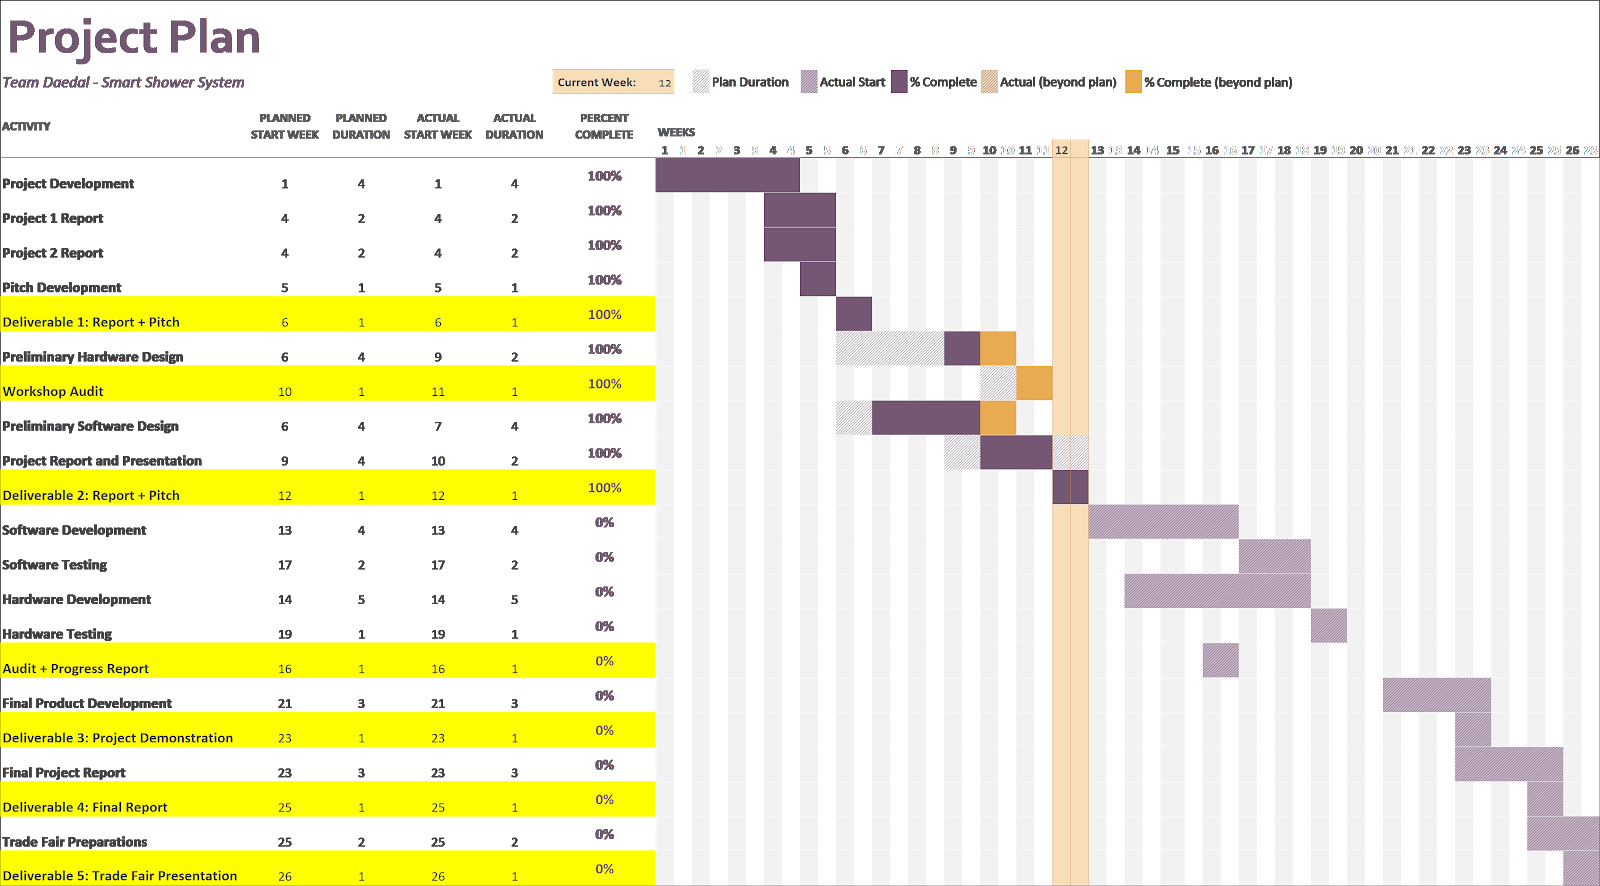
\includegraphics[width=\linewidth]{img/Gantt_Chart_Final.png}
                \caption{Project Plan Gantt Chart}
            \end{figure}
            \paragraph{}
                From the figure above (larger version available at Figure 24 in the appendix), it can be seen that the project plan so far has not gone as initially planned. This is mainly due to the meeting 
                with Enware that was held in week 8, which drastically changed our project direction. Initially the plan was to contact the Industry sponsor 
                immediately after project approval to gain insight. Due to complications in initial communication with Enware, a meeting could not be organised 
                until 3 weeks after approval.
            \paragraph{}
                This setback was unexpected, but when the initial design was brought up with Enware in the first meeting, it was revealed that the system is already 
                under development. Subsequently, a team meeting was held to address the new information from Enware.The team decided that major changes were to be 
                made to the initial plan. This caused the delay in starting the preliminary hardware design.
            \paragraph{}
                The effect of this was that the team had to work twice as hard to complete the preliminary hardware design before week 11. Since the initial plan 
                expected everything to be completed early, the deadline was still met despite finishing later than expected.
            \paragraph{}
                From the software side of the project, since receiving the information from Enware not much has changed in the design. Initially the team agreed to 
                spend a few weeks gaining familiarity with the Raspberry Pi and learning about Python. Pseudo code was required for the report in week 12. The plan 
                was to have it completed by week 10, but, due to the lack of knowledge of the systems involved, extra time was required. Since the expected deadline 
                was quite ambitious, despite the extra week required, the software team is still on track with expected progress.
        \subsection{Budget Analysis}
            \paragraph{}
                The major costs related to the smart shower project have been accrued due to the research and development time supplied by team members. The other 
                major cost being hardware components required for testing. Initially 6 hours per team member per week was allocated but due to time challenges each 
                team member only supplied 3 hours/week. This has resulted in 72 hours saved under the expected time. A single hour of work is billed at \$45/hour. 
                There has currently been 216 hours accrued on the project, bringing the total billed hours to \$9720 and giving a cost savings of \$9720. Furthermore, 
                the team saved an additional \$350 from consultation and workshop time due to collaboration with other teams.
            \paragraph{}
                The estimation for hardware pricing was \$215.99 from the initial project pitch. After meeting with Enware and finalising the project scope, this cost 
                has been reduced to \$179.52, resulting in approximately a \$36 saving. Deadal was given a budget of \$350 of which \$170.48 is remaining, to be used 
                for unforseen circumstances if required. 
            \paragraph{}
                The table below indicates detailed costs on the works carried out. The team used equal amounts in time with both hardware and software related work. 
                The most amount of time was involved in the team meetings on making decisions. This is largely due to indirection resulting from difficulty getting 
                ahold of the client. The team handled the decision making well and made up for lost time while also saving close to 50\% of the cost. 

            \begingroup
                \centering
                \begin{flushleft}
                \resizebox{\linewidth}{!} {
                    \begin{tabular}{| m{0.2\linewidth} | m{0.16\linewidth} | m{0.16\linewidth} | m{0.16\linewidth} | m{0.16\linewidth} | m{0.16\linewidth} |}
                        \hline
                        \textbf {Expense} & \textbf {Expected Hours} & \textbf {Actual Hours} & \textbf {Cost/Hour} & \textbf {Expected Subtotal} & \textbf {Actual Subtotal} \\ \hline
                        Research and development & 432 & 216 & \$45 & \$19 440 & \$9 720 \\ \hline
                        Consultation & 3 & 0.5 & \$60 & \$180 & \$30 \\ \hline
                        Workshop time & 3 & 0 & \$75 & \$225 & \$0 \\ \hline
                        & & & \textbf {Total} & \textbf {\$20 065.00} & \textbf {\$9 750.00} \\
                        \hline
                    \end{tabular}
                }
                \end{flushleft}
                \captionof{table}{Projected vs Actual Expenses}\label{tbl:expensestable}
            \endgroup
            \begingroup
                \centering
                \begin{flushleft}
                \resizebox{\linewidth}{!} {
                    \begin{tabular}{| m{0.2\linewidth} | m{0.16\linewidth} | m{0.16\linewidth} | m{0.16\linewidth} | m{0.16\linewidth} | m{0.16\linewidth} |}
                        \hline
                        \textbf {Work area} & \textbf {March} & \textbf {April} & \textbf {May} & \textbf {Subtotal} & \textbf {Cost} \\ \hline
                        Hardware & 15 & 16 & 30 & 61 & \$2 745 \\ \hline
                        Software & 15 & 13 & 32 & 60 & \$2 700 \\ \hline
                        Deliverables & & 10 & 15 & 25 & \$1 125 \\ \hline
                        Administration & 1 & 1.5 & 2 & 4.5 & \$202.50 \\ \hline
                        Meetings & 10 & 20 & 35.5 & 65.5 & \$2 947.50 \\ \hline
                        & & & \textbf {Total} & \textbf {216} & \textbf {\$9 750.00} \\
                        \hline
                    \end{tabular}
                }
                \captionof{table}{Time spent across work areas each month}\label{tbl:workareastable}
                \end{flushleft}
            \endgroup
            \begingroup
                \centering
                \begin{flushleft}
                    \resizebox{\linewidth}{!} {
                        \begin{tabular}{| m{0.2\linewidth} | m{0.16\linewidth} | m{0.16\linewidth} | m{0.16\linewidth} | m{0.16\linewidth} | m{0.16\linewidth} |}
                            \hline
                            \textbf {Item} & \textbf {Part Number} & \textbf {Supplier} & \textbf {Quantity} & \textbf {Unit Price} & \textbf {Total Price} \\ \hline
                            Water turbine & SEN0029 & Core Electronics & 3 & \$15.81 & \$47.43 \\ \hline
                            Peltier Thermo-Electric Module & ADA1330 & Core Electronics & 2 & \$22.70 & \$45.40 \\ \hline
                            Banana Socket RED & CEO5221 & Core Electronics & 8 & \$0.46 & \$3.68 \\ \hline
                            Banana Socket BLACK & CEO5165 & Core Electronics & 8 & \$0.46 & \$3.68 \\ \hline
                            Wattmeter & ADA3624 & Core Electronics & 1 & \$47.40 & \$47.40 \\ \hline
                            Load Resistor & RR0565 & Jaycar & 1 & \$0.55 & \$0.55 \\ \hline
                            Raspberry Pi Zero W & CEO5324 & Core Electronics & 1 & \$21.40 & \$21.40 \\ \hline
                            SD Card & SDSQ16GB & Officeworks & 1 & \$9.98 & \$9.98 \\ \hline
                            & & & & \textbf {Total} & \textbf {\$179.52} \\
                            \hline
                        \end{tabular}
                    }
                    \captionof{table}{Budget for parts to be purchased}\label{tbl:budgettable}
                \end{flushleft}
            \endgroup
            \subsubsection{Cost and Profit Analysis}
                \paragraph{}
                    As we are working in conjunction with Enware, we have additional resources at hand besides the \$350. These resources that are provided are not a 
                    direct cost to the team, but are required to be acknowledged for deciding on a price to market the device.
                \paragraph{}
                    The production of a single prototype will cost \$179.52 in hardware. This cost does not include individual hourly costs. By adding a margin to this 
                    we can sell the final product for \$229.99. From our budgeting, it is predicted that \$19680 will be spent on labour cost (both autumn and spring 
                    session combined). From our market research, it has been determined that 850 to 1000 products can be sold in the first financial year of the final 
                    product. Taking into consideration marketing, an additional \$5000 is required per year. Having a margin of \$50.47 per product, the breakeven point 
                    is realised at 489 products. If projected sales are met, we are looking at a profit of \$18219.5 to \$25790 in the first year.
                \paragraph{}
                    To stay competitive in today's market the price of our product should stay well within the market range\cite{smart_home}. The market analysis showed us the cheapest 
                    product is provided by Moen and costs \$1160 excluding plumbing costs, as it can only be installed professionally. The next product competing with 
                    Daedals smart shower is envisioned by Livin Shower for \$600, which is still under Research and Development(R\&D). We have set a margin of over 50\% 
                    difference in product cost making it viable and highly desirable for everyday families and homes.
        \subsection{Workshop Audit}
            \textbf{Aim:}
            \paragraph{}
                The aim of the workshop is to prove that our design is feasible and within our scope.
            \newline
            \textbf{Discussion:}
            \paragraph{}
                After discussing our design with the workshop officer, there were three key issues that were brought up in terms of the hardware aspect of our project:
                \begin{enumerate}
                    \item The design of the thermoelectric generator testing layout.
                    \item The power requirements of our prototype design.
                    \item The presentation of the prototype at the innovation fair.
                \end{enumerate}
            \textbf{Results:}
            \paragraph{}
                The outcome of the key points was:
                \begin{enumerate}
                    \item To successfully generate power using the thermoelectric generator, we will have to organise for one of the mechanical workshop machinists 
                    to make a part for us out of aluminium. This can be done once we physically have our thermoelectric generator, as we will then be able to design 
                    the part to fit around it.
                    \item Since the power requirements are quite low for our design, the workshop will not need to approve of any power sources we might need, as 
                    they will not be 240V.
                    \item The presentation of the project will be a major issue due to the large amounts of water required to properly demonstrate our prototype. 
                    The safety aspect of this, i.e. water leaks and electrical cables, means that the best way to demonstrate at the trade fair will be through a 
                    pre-recorded video. This isn’t the ideal method of demonstration, but, given the circumstances it will have to suffice, as we will not have access 
                    to water outlets at the trade fair.
                \end{enumerate}
        \subsubsection{Saftey Considerations}
            \paragraph{}
                The major requirement of shower products is to give users a safe and comfortable feeling. To meet these goals, the software has to work with the 
                hardware in an expected manner.
            \paragraph{}
                First of all, in order to prevent users from being scalded, the software must be robust and enforce strict safety measures in temperature controls. 
                Comprehensive testing is required to ensure that under no circumstances, the users’ safety is compromised. In terms of hardware, we will ensure 
                sensitivity and stability of the electrical connections before assembly of the controller.
            \paragraph{}
                In addition, we also consider the user's control experience, so we have designed default water temperature function and the last water temperature 
                function.  After which the user can adjust the temperature as needed (we have set the temperature range in the database to prevent the water 
                temperature from being too high).
            \paragraph{}
                All components of the shower system must be waterproof to prevent possible electrocution and malfunctions. This is the major safety concern for the 
                design.
            
    \newpage
    \section{Sustainabliity and Ethics}
        \subsection{Sustainabliity}
            \paragraph{}
                In this day and age, sustainability is an important part that is considered in all areas of creation of product. 
            \paragraph{}
                As modern technology is evolving into a sustainability focused mindset, our design follows suit. The materials required to produce the 
                design must be taken into consideration. Similarly, water usage is monitored through the application of the device. This is due to the 
                importance of conserving Earth’s natural resources.
            \paragraph{}
                Daedal aims to focus on making the system, designed by Enware, independent of the electrical mains system. This is achieved by generating 
                electricity from the water passing through the shower plumbing, as well as the temperature difference between the pipes. By shifting the system 
                off the electrical grid, this will reduce the impact on natural resources.
            \paragraph{}
                A part of the system is to make the user more conscience of their water usage. Since clean drinkable water is a finite resource, it is imperative 
                that society minimises the use of water as much as possible. 
            \paragraph{}
                The results of the hardware system will determine if it is feasible to remove the system off the electrical grid. If it is not, Daedal aims to 
                reduce the burden the system creates by placing a subsystem onto a battery.
            \paragraph{}
                The aim of this product in terms of Deadal’s development is to create a product that is affordable. Due to the wide use of showers throughout the 
                world, to create both social and economical sustainability it is vital that the product is accessible for everyone.
        \subsection{Ethics}
            \paragraph{}
                Ethics is a highly considered aspect of design. It is a focus of Enware’s as a company, and therefore ours. We aim to develop our product to benefit 
                those that are mentally or physically disadvantaged. This is to be done by assisting Enware and their direction of interest with a wireless application 
                control of their system. This is to work alongside Enware’s current control methods and offer a more modern method of controlling the shower.
            \paragraph{}
                Enware has developed tap sensors to visually assist with determining the temperature of  the water output. Daedal aims to further this by controlling 
                the temperature and pressure from a wireless application. This aims to give further assistance and clarity to those disadvantaged. Also it can assist 
                those caring for the disadvantaged by giving them a method to easily control and adjust the water of the shower from outside the shower itself.
            \paragraph{}
                The inclusion of settings forced onto the system by an external application allows many parameters to be set. This is highly beneficial to those that 
                need to set temperature and pressure to stop harm occurring. The main application for this is controlling the temperature for children and the elderly, 
                who are more prone to accidentally changing shower temperature.
            \paragraph{}
                Another key ethical issue is independence. A study has shown that 17.5\% of 60-69 year olds, 24.3\% of 70-79 year olds and 33.8\% of 80+ year old 
                Australians live alone\cite{living_alone}.Of those living alone, there are many who may have mild-severe cognitive disabilities which may impact them 
                on a daily basis. Our product utilises a behavioural notification system, which can alert a loved one or a carer if the user is not showering for an 
                irregular amount of time. Purely for hygienic reasons, it is good to make sure the user is showering, but this may also be indicative of a larger issue. 
                The notification system is crucial for allowing users to have independence, while also having peace of mind in case something goes wrong.
            \paragraph{}
                In addition to the safety benefits provided by our product, it is also key to note the environmental benefits that the product is looking to achieve. 
                The constantly updated water usage data on the user interface, as well as notifications to the user will maintain the users’ knowledge of their water 
                usage habits. By allowing users to set water usage goals, and keeping them updated on their progress, it will further enforce in their mind the 
                importance of minimising time in the shower.
        
    \newpage
    \section{Conclusions and Recommendations}
        \subsection{Conclusion}
            \paragraph{}
                The main focus for Daedal is to further the existing product’s capabilities in both hardware and software. For hardware, the task is to research and 
                explore the possibility of an independently powered system by utilising waste energy produced during showers, through the use of thermoelectric and 
                hydroelectric generators. This system will be examined with a test layout designed and developed in-house. The team is confident that enough energy can 
                be generated ahead of testing, as the required power is much less than anticipated. Regarding software, Daedal will be further extending the smart 
                functions of the product by developing digital water monitoring through sensors, data logging, UX/UI and wireless control of the system using a 
                Raspberry Pi Zero module or a smart phone application. 
            \paragraph{}
                During the initial stage, there were some unexpected setbacks which slowed down the team’s progress. However the team is confident of finishing the 
                required testing and software development come the spring session. Once the product is finalised, Daedal can then focus on troubleshooting and 
                perfecting the system both hardware and software-wise.
        \subsection{Recommendations}
            \spacing{1.5}
            \begin{enumerate}
                \item Considering that the team is working a little slower than expected, and we have obtained the relevant model from Enware. We can continue our 
                software design and hardware assembly for some time during the coming holiday.
                \item Because teamwork is lagging behind expectations, we can try to take some time to improve the project management process in order to match project 
                schedule and ensure cohesion and efficiency of the whole team.
                \item Team projects may stall at some point because all members lack expertise, such as programming. In this case, we can consider outsourcing work 
                to experts who can accomplish tasks faster, rather than letting someone in the team learn all the information they need.
            \end{enumerate}
        \spacing{1.5}

    \newpage
    \section{References}
        \printbibliography

    \newpage
    \appendix
        \section{Project Plan Gantt Chart (Full Size)}
            \begin{figure}[H]
                \centering
                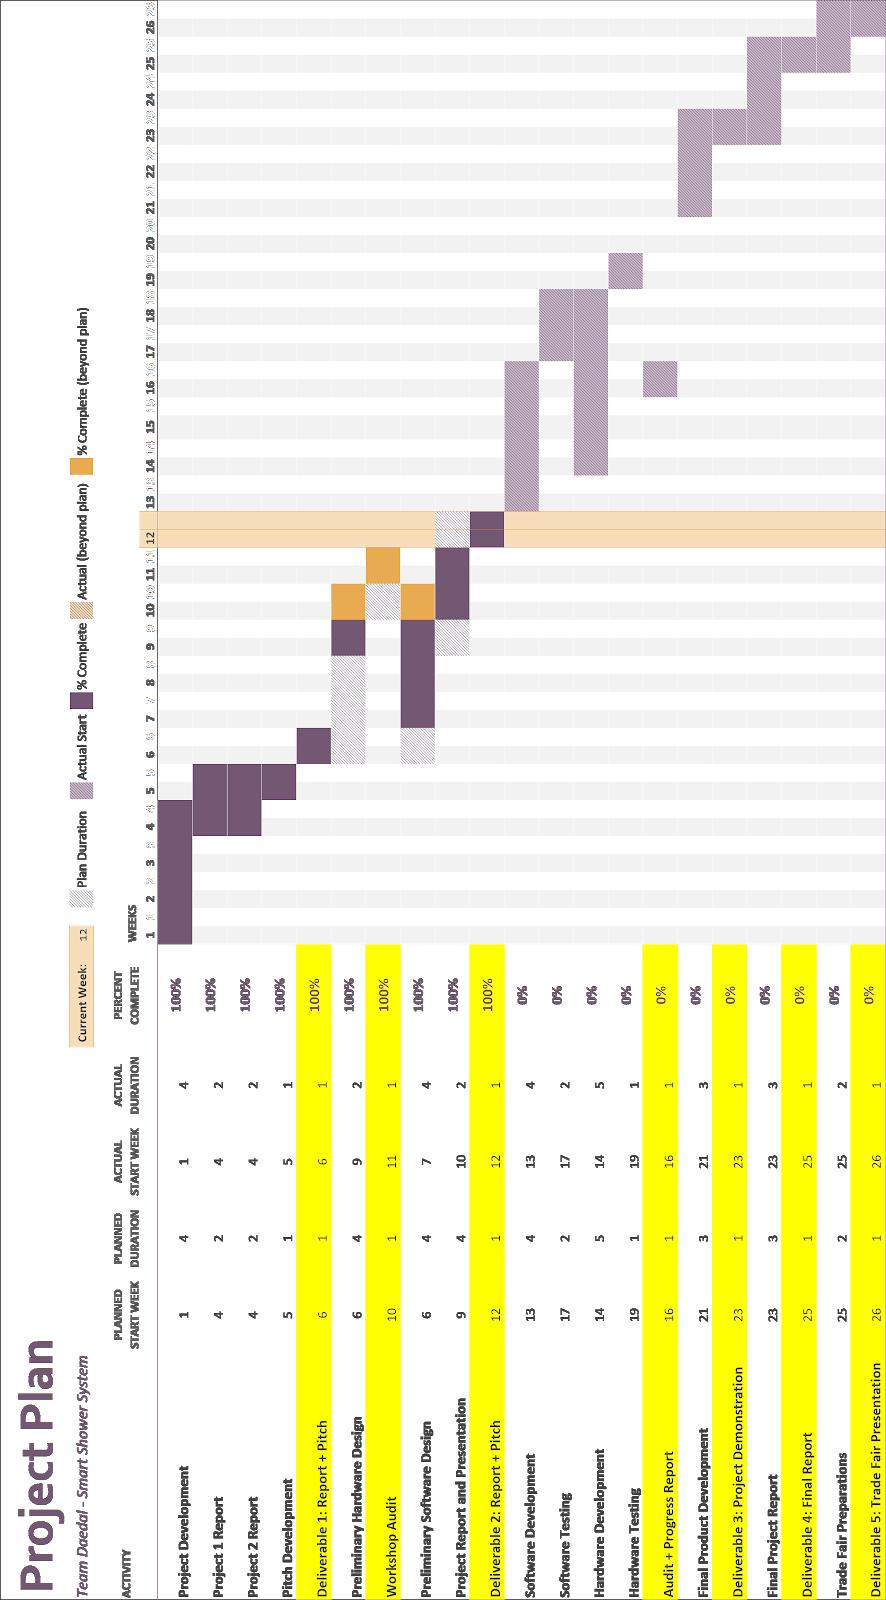
\includegraphics[width=0.8\linewidth]{img/Gantt_Chart_Final_Vertical.png}
                \caption{Project Plan Gantt Chart (Full Size)}
            \end{figure}
        \newpage
        \section{Completed Code Examples}
            \footnotesize
            \spacing{1}
            \begin{figure}[H]
                \begin{lstlisting}
    var http = require('http');
    var fs = require('fs');
    var mysql = require('mysql');

    // var con = mysql.createConnection({
    //     host: "localhost",
    //     user: "root",
    //     password: "mysql"
    // });

    var server = http.createServer(function (request, response) {
        console.log(request.url);
        if (request.url == "/") {
            fs.readFile('./index.html', function(err, data) {
                response.setHeader('Content-type', 'text/html');
                response.write(data);
                response.end();
            });
        } else {
            fs.readFile('./' + request.url, function(err, data) {
                if (!err) {
                    var dotoffset = request.url.lastIndexOf('.');
                    var mimetype = dotoffset == -1
                                    ? 'text/plain' : {
                                        '.html' : 'text/html',
                                        '.ico' : 'image/x-icon',
                                        '.jpg' : 'image/jpeg',
                                        '.png' : 'image/png',
                                        '.css' : 'text/css',
                                        '.js' : 'text/javascript',
                                        '.ttf' : 'font/ttf',
                                        '.woff' : 'font/woff',
                                        '.svg' : 'image/svg+xml',
                                        '.map' : 'text-plain'
                                        }[ request.url.substr(dotoffset) ];
                    response.setHeader('Content-type' , mimetype);
                    response.end(data);
                } else {
                    response.writeHead(404, "Not Found");
                    response.end();
                }
            });
        }
    }).listen(8080);
                \end{lstlisting}
                \caption{Server setup javascript code example}
            \end{figure}
            \normalsize
            \spacing{1.5}
            \footnotesize
            \spacing{1}
            \begin{figure}[H]
                \begin{lstlisting}
    var attempt = 3; // Variable to count number of attempts.

    // Below function Executes on click of login button.
    function validate(){
        var username = document.getElementById("username").value;
        var password = document.getElementById("password").value;

        if ( username == "Formget" && password == "formget#123") {
            alert ("Login successfully");
            window.location = "success.html"; // Redirecting to other page.
            return false;
        } else {
            attempt --;// Decrementing by one.
            alert("You have left " + attempt + " attempt;");

            // Disabling fields after 3 attempts.
            if( attempt == 0){
                document.getElementById("username").disabled = true;
                document.getElementById("password").disabled = true;
                document.getElementById("submit").disabled = true;
                return false;
            }
        }
    }
                \end{lstlisting}
                \caption{JavaScript Login Form Example\cite{login_form}}
            \end{figure}
            \normalsize
            \spacing{1.5}

        \newpage
        \section{Individual Performance Reviews}
            \subsection{Thomas Battye-Smith (5570001)}
                \paragraph{}
                    From the start of the semester my contributions include:
                    \begin{itemize}
                        \item The design of the control system for the ISD Smart Battery. This included researching various methods for battery voltage monitoring, 
                        coulomb counting and cell balancing methods.
                        \item I completed the electrical schematics and hardware list for the project pitch report ISD Smart Battery. Additionally, I completed the 
                        first half of the presentation for ISD Battery.
                        \item Upon being assigned to Enware Smart Shower project, I went to the initial meeting to gather information and direction. 
                        \item For the autumn session report, I have completed the introduction, electrical schematic, hardware (generator) overview.
                        \item Additionally I met with Wayne Ireland for the WHS assessment.
                    \end{itemize}
            \subsection{Quang Hung Pham (5560512)}
                \paragraph{}
                    From the beginning of the project, my contributions so far include: research on measuring the battery’s State of Charge and LED output for the 
                    smart drone battery project for Industry Spec Drones, and battery parts sourcing, which included the cells we were going to use for our project 
                    should it be chosen, and a battery monitoring IC. I also prepared and presented the second half of the smart drone battery pitch in Week 6.
                \paragraph{}
                    For our chosen project (Enware smart shower system), my role as part of the hardware team is to research and gain an understanding in thermoelectric 
                    and hydroelectric system. For the report, I did Market Analysis which included marketing summary, strategy, competitor analysis, product advantages 
                    and disadvantages, and in addition, the report conclusion.
            \subsection{Ilija Babic (5777446)}
                \paragraph{}
                    At the start of the project I was tasked with the market analysis of the smart drone battery pitch, and the user interface for our smart shower 
                    pitch. Since our smart shower system was approved as our project, my role changed to software engineer. My main task for the first few weeks was 
                    to gain an understanding of the raspberry pi and python. I then went to the initial meeting with Enware to discuss our project, and from that 
                    meeting it was decided that our whole project needed to change. As we approached the report deadline, I organised another meeting with Enware to 
                    discuss the software aspect of our product, and obtain their prototype, along with the necessary documentation. I also in the meantime completed 
                    the pseudocode for the data logging and user notifications, as well as elaborating on the ethics of our design from the software perspective. I 
                    then went with the group to the workshop audit, and afterwards completed the workshop audit report. After completing all of that, I then did the 
                    Gantt chart and progress report, and started to work on our group presentation.
            \subsection{Yuhao Cui (6101422)}
                \paragraph{}
                    My contributions so far this semester have included:
                    \begin{enumerate}
                        \item After consulting the relevant information, the key requirements and problems of UAV smart battery are summarized and simply answered.
                        \item The budget estimate of ISD smart battery project is completed, and the input function of Enway smart shower system is designed.
                        \item Responsible for completing the second half of the speech on smart shower system(6th week).
                        \item After the smart shower system was selected as the project of our team, I was responsible for writing the JAVA code of controlling the running time.
                        \item Participated in the second meeting with Enware, discussed the software aspect of our product, and got their model and related documents.
                        \item Participate in workshop audit with team members.
                        \item Completed “Safety Consideration” and “Recommendation” for the autumn session report(12th week).
                    \end{enumerate}
            \subsection{Lachlan Fowke (5065549)}
                \begin{itemize}
                    \item Initially team leader, sustainability and ethics for first choice project and editor for second project proposal report
                    \item Set up and attended first meeting with Enware
                    \item Design CAD drawing of testing design
                    \item Hardware overview, explained the design, test procedures, expected results, sustainability, developed initial ethics and assisted in editing 
                        for the autumn report
                    \item Lead in mechanical components
                    \item Presenting hardware section of end of autumn presentation.
                \end{itemize}
            \subsection{Timothy Martin (5726803)}
                \paragraph{}
                    In the Autumn Session, I have contributed to my team in various ways. At the beginning of the semester, for the first deliverable I invented the 
                    idea for a Smart Shower project which we ended up using. I also helped my team in creating the first deliverable by providing the target 
                    specification, project plan (including the data flow diagram and a block diagram of the proposed design), a section on the capabilities of the 
                    team and an estimated full costing for the project.
                \paragraph{}
                    For the second deliverable I assisted in parts of the creation of the presentation and presented the first half of the Smart Shower project to the 
                    board and my peers.
                \paragraph{}
                    Since these deliverables I have acted as project manager for our team by writing meeting minutes, ensuring all team members are aware of their 
                    roles and are progressing in their sections of the project, having good general knowledge on the overall design and plans for our project and 
                    making decisions relating to the software aspects of the project in regards to chosen language, platform and as well as ensuring we are compatible 
                    with the current prototype from Enware.
                \paragraph{}
                    For the second deliverable report I have produced the server setup and interface design aspects of the report, filling in summaries and other more 
                    general areas of the report, managing the references and formatting the report using LaTeX to ensure a nice, professional document is produced at 
                    the end.
                \paragraph{}
                    For the continuation of this project I shall be concentrated on the software by using my existing experience with, both the language we are using 
                    and the platforms we are building upon to assist the less experienced members of our software team to learn how to program the software solutions 
                    we will be employing. I also intend to do some of the grunt-work for both the hardware and software portions of the project, so that I may gain 
                    kills and experience working in areas where other members of my team are more experienced.
            \subsection{Amalesh Nagenthiran (4184312)}
                \paragraph{}
                    At the start of the project my roles was to research and write the report on the inputs of the battery. Researched ways to measure the inputs 
                    needed, best way to connect the battery (series or parallel), calculations on suitable battery charger size. For our wild card project, the team 
                    agreed on Tim’s smart shower system. My role for the wildcard was sustainability and ethics. For the pitch in deliverable two I designed the 
                    proposal for both the smart shower and drone battery for the presentation
                \paragraph{}
                    Since our smart shower system was approved as our project, my role changed to software engineer. My main task for the first few weeks was to gain 
                    an understanding of the raspberry pi and python and after the team went to the initial meeting with Enware we realised the whole project needed 
                    to change and I started understanding node.js and javascript and researched on understanding how to read from the raspberry pi pins with the 
                    aforementioned software, as we approached the project report deadline I went to the software team meeting with Enware to get a better understanding 
                    of the product and the workshop audit with the team, in the meantime developed the functions for the smart shower system along with their pseudocode 
                    and also a sample code for the login verification. I also designed a prototype user interface to be able to visualise the buttons and their functions 
                    which could also be used on mobile by clients to understand the system and we will be using the interface video in the project presentation. I 
                    completed the User interface function design, Marketing strategy, commercialisation strategy and the resources and budget part of the report and 
                    will be going over the requirements and document checking to make sure we aren’t missing anything. For the final presentation we will be using the 
                    same file that I made for the smart shower pitch which will retain most of the information and will start editing it. I will also be delivering part 
                    of the presentation for deliverable 4.
\end{document}